% LTeX: language=en-US
\documentclass[handout,usepdftitle=false,xcolor=dvipsnames,aspectratio=169]{beamer}
%\documentclass[beamer,usepdftitle=false,xcolor=dvipsnames,aspectratio=169]{beamer}
%\documentclass[trans,notes=show,usepdftitle=false,aspectratio=169]{beamer}


\usepackage[english]{babel}
\usepackage{iftex}
\ifPDFTeX
\usepackage[T1]{fontenc}
\usepackage[utf8]{inputenc}
\usepackage{lmodern}
\else
\usepackage{fontspec}
\defaultfontfeatures{Ligatures=TeX}
\setmainfont{Latin Modern Roman}
\setsansfont{Latin Modern Sans}
\setmonofont{Latin Modern Mono}
\usepackage{newunicodechar}
\newfontfamily\unicodeSymbolFont{Segoe UI Symbol}[
  BoldFont=Segoe UI Symbol,
  ItalicFont=Segoe UI Symbol,
  BoldItalicFont=Segoe UI Symbol
]
\newunicodechar{⟂}{{\unicodeSymbolFont ⟂}}
\fi
\usepackage{amsmath,amsfonts}
\usepackage{booktabs,multirow,xcolor,colortbl}
\usepackage{bm}%to use a more powerful version of \boldsymbol
\usepackage{fvextra}
\usepackage{csquotes}
\usepackage{textcomp}
\ifPDFTeX
\DeclareUnicodeCharacter{27C2}{\ensuremath{\perp}}
\fi

\newcommand{\AllSample}{ \mathcal Y^T }

\usepackage[citestyle=authoryear-comp,bibstyle=../Preamble/mystyle_lowercase,maxbibnames=5,minbibnames=1,maxnames=2, minnames=1,datezeros=false,date=long,isbn=false,url=false,backend=biber,useprefix=true]{biblatex}
\addglobalbib{../Preamble/Macro_database_biblatex.bib}	

\usepackage{upquote}
\usepackage{ragged2e}
\usepackage{microtype}

\usepackage{multimedia}
\usepackage{graphicx}
\usepackage[export]{adjustbox}
\usepackage{epstopdf}
\usepackage[labelfont=bf,format=hang, figurename=Fig.]{caption}
\usepackage[subrefformat=parens,labelformat=empty]{subcaption}
\usepackage{pgfpages} % for multiple-screen presentations

\usepackage{array}

\newcolumntype{L}[1]{>{\RaggedRight\let\newline\\\arraybackslash\hspace{0pt}}m{#1}}
\newcolumntype{C}[1]{>{\centering\let\newline\\\arraybackslash\hspace{0pt}}m{#1}}
\newcolumntype{R}[1]{>{\raggedleft\let\newline\\\arraybackslash\hspace{0pt}}m{#1}}
%https://tex.stackexchange.com/questions/12703/how-to-create-fixed-width-table-columns-with-text-raggedright-centered-raggedlef


%%% use serif font for math
\usefonttheme[onlymath]{serif}

%%% define blue highlighting
\newcommand{\highlight}[1]{{\color{blue}{#1}}}

%%%% define command for setting sources

\newcommand{\Source}{}

%%%
\beamertemplatenavigationsymbolsempty


%%% define themes
\usetheme{Boadilla}
\usecolortheme{rose}
\usecolortheme[named=blue]{structure}

\newcommand\textbox[1]{%
  \parbox{.333\textwidth}{#1}%
}

\setbeamertemplate{sections/subsections in toc}[sections numbered]


%%%% set coloring in  foot and head
\setbeamercolor{alerted text}{fg=red!80!black}
\setbeamertemplate{enumerate items}[default] % numbers enumerate items without encircling them
\setbeamertemplate{itemize items}[ball] % numbers enumerate items without encircling them
\setbeamercolor{section in head/foot}{fg=black, bg=white}
\setbeamercolor{subsection in head/foot}{fg=black, bg=white}
\setbeamercolor{title}{fg=black}
\setbeamercolor{subtitle}{fg=blue}

\setbeamertemplate{caption}[numbered]

%%% set overlays as default
\beamerdefaultoverlayspecification{<+->}

%%%% settings for output mode

\mode<beamer>
{
%\setbeameroption{show notes on second screen=right}
}

\mode<trans>
{\renewcommand{\highlight}[1]{{\textbf{#1}}}}


\mode<handout>
{
\renewcommand{\highlight}[1]{{\textbf{#1}}}
%\pgfpagesuselayout{4 on 1}[a4paper,border shrink = 5mm,landscape]
%\setbeamercolor{background canvas}{bg=black!5}
}


%%% define Exercise counter
\newcounter{Exercise}
\resetcounteronoverlays{Exercise}
\setcounter{Exercise}{0}
\newcommand{\Exercise}{\refstepcounter{Exercise}\emph{\structure{Übung \theExercise}: }}

%%%% define environments for theorems etc and make them numbered
\setbeamertemplate{theorems}[numbered]

\newtheorem{assum}{Assumption}
\setbeamertemplate{assum}[numbered]

\newtheorem{defin}{Definition}
\setbeamertemplate{defin}[numbered]

\newtheorem{propos}{Proposition}
\setbeamertemplate{propos}[numbered]


%%%% Make Parts show up in TOC
\makeatletter
\AtBeginPart{%
  \addtocontents{toc}{\protect\beamer@partintoc{\the\c@part}{\beamer@partnameshort}{\the\c@page}}%
}
%% number, shortname, page.
\providecommand\beamer@partintoc[3]{%
  \ifnum\c@tocdepth=-1\relax
    % requesting onlyparts.
    \makebox[6em]{#1.} #2
    \par
  \fi
}
\define@key{beamertoc}{onlyparts}[]{%
  \c@tocdepth=-1\relax
}
\makeatother%

%%%% fix bug in beamer package with note itemize
%%% http://tex.stackexchange.com/questions/1480/changing-the-textwidth-of-the-notes-in-beamer-repost-from-so
\makeatletter
\defbeamertemplate{note page}{infolines}
{%
  \vskip.75em
  \nointerlineskip
  \begin{minipage}{\textwidth} % this is an addition
  \footnotesize \insertnote
  \end{minipage}               % this is an addition
}
\makeatother

\setbeamertemplate{note page}[infolines]


\newcommand{\backupbegin}{
   \newcounter{framenumberappendix}
   \setcounter{framenumberappendix}{\value{framenumber}}
}
\newcommand{\backupend}{
   \addtocounter{framenumberappendix}{-\value{framenumber}}
   \addtocounter{framenumber}{\value{framenumberappendix}}
}

\hypersetup{bookmarksnumbered=true,naturalnames=true,pdfhighlight=/N,citebordercolor={1 1
1},linkbordercolor={1 1 1},colorlinks=true,anchorcolor=black,linkcolor=blue,citecolor=green,urlcolor=green,
pdfpagemode=UseOutlines,breaklinks=true,
pdfkeywords=Dynare, pdfsubject=Dynare,pdfstartpage=1} %pdfpagemode=fullpage

\usepackage[copyright]{ccicons}

\usepackage{tikz,pgfplots}
\pgfplotsset{compat=1.18}
\usetikzlibrary{arrows,calc,decorations.pathreplacing,decorations.shapes}
\pgfdeclarelayer{background}
\pgfdeclarelayer{foreground}
\pgfsetlayers{background,main,foreground}

\usepackage{relsize}
\newcommand\LM{\ensuremath{\mathit{LM}}}
\newcommand\IS{\ensuremath{\mathit{IS}}}
\DeclareMathOperator{\std}{std}


\setbeamertemplate{footline}{
\begin{beamercolorbox}{subsection in head/foot}
\insertsectionnavigationhorizontal{.95\textwidth}{\hskip0pt
\hfill}{\hfill \insertframenumber /\inserttotalframenumber}
\end{beamercolorbox}
}

\newenvironment{witemize}{\itemize\addtolength{\itemsep}{8pt}}{\enditemize}
\newenvironment{wenumerate}{\enumerate\addtolength{\itemsep}{8pt}}{\endenumerate}

\usepackage[]{minted}
\usepackage{tcolorbox}
\usepackage{etoolbox}
\BeforeBeginEnvironment{minted}{\begin{tcolorbox}[boxsep=0mm]}%
\AfterEndEnvironment{minted}{\end{tcolorbox}}%

\AtBeginEnvironment{minted}{%
  \renewcommand{\fcolorbox}[4][]{#4}}  


\title[]{\textbf{Advanced Dynare\\}
\medskip{Chapter III}\\
\emph{The Dynare macroprocessor}
}

\author{Johannes Pfeifer}
\input{../date_place.txt}

\AtBeginSection[]
{
  \begin{frame}
    \frametitle{Outline}
    \tableofcontents[currentsection]
  \end{frame}
}

\begin{document}

\begin{frame}<4->
  \titlepage
  \begin{columns}[T]
    \column{0.3\textwidth}
    \column{0.09\textwidth}

    \ccbysa
    \column{0.61\textwidth}
    \tiny
    Copyright © 2008-2025 Dynare Team \\
    License: \href{http://creativecommons.org/licenses/by-sa/4.0/}{Creative
      Commons Attribution-ShareAlike 4.0}
  \end{columns}
\end{frame}

\begin{frame}
  \frametitle{Outline}
  \tableofcontents
\end{frame}

\section{Overview}

\begin{frame}
  \frametitle{Motivation}
  \begin{witemize}
    \item The \textbf{Dynare language} (used in \texttt{.mod} files) is well suited for many economic models
    \begin{witemize}
      \item It's a markup language that defines models
      \item but lacks programmatic element
    \end{witemize}
    \item The \textbf{Dynare macro language} adds programmatic element
    \begin{witemize}
      \item Introduces conditionals, loops, and other simple programmatic directives
      \item Used to speed up model development
      \item Useful in various situations
      \begin{witemize}
        \item Multi-country models
        \item Creation of modular \texttt{.mod} files
        \item Variable flipping
        \item Conditional inclusion of equations
        \item \ldots among others
      \end{witemize}
    \end{witemize}
  \end{witemize}
\end{frame}

\begin{frame}
  \frametitle{Design of the macro language}
  \begin{witemize}
    \item The Dynare macro language provides a set of \textbf{macro commands} that can be used in \texttt{.mod} files
    \item The macro processor transforms a \texttt{.mod} file with macro commands into a \texttt{.mod} file without macro commands (doing text expansions/inclusions) and then feeds it to the Dynare parser
    \item Key point: the macro processor only performs \textbf{text substitution}\\
    $\rightarrow$ objects computed in later steps are not available yet and cannot be conditioned on
  \end{witemize}
\end{frame}

\begin{frame}
  \frametitle{Dynare Flowchart}
  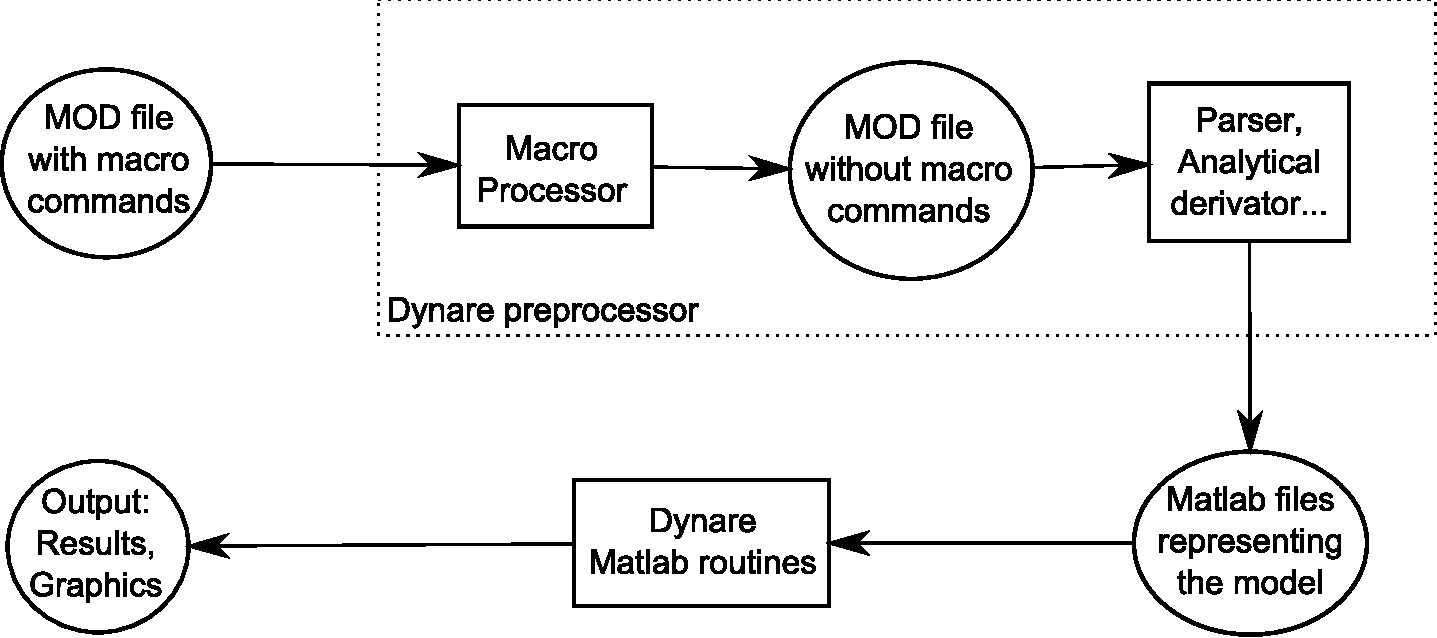
\includegraphics[width=0.95\linewidth]{figures/new-design.pdf}
\end{frame}

\section{Syntax}

\begin{frame}[fragile]
  \frametitle{Macro Directives}
  \begin{witemize}
    \item Directives begin with: \verb+@#+
    \item A directive gives instructions to the macro processor
    \item Main directives are:
    \begin{itemize}
      \item file inclusion: \verb+@#include+
      \item definition of a macro processor variable or function: \verb+@#define+
      \item conditional statements: \verb+@#if/@#ifdef/@#ifndef/@#else/@#elseif/@#endif+
      \item loop statements: \verb+@#for/@#endfor+
    \end{itemize}
    \item Most directives fit on one line\\
    $\rightarrow $ two backslashes (\textit{i.e.} \verb+\\+) at end of line indicate that directive is continued
    \item Directives are not terminated with a semicolon
  \end{witemize}
\end{frame}

\begin{frame}
  \frametitle{Values and types}
  \begin{itemize}
    \item The macro processor can handle values of 5 different types:
          \begin{enumerate}
            \item boolean (logical value, true or false)
            \item real (double precision floating point number)
            \item string (of characters)
            \item tuple
            \item array
          \end{enumerate}
    \item Preprocessor is type sensitive!
    \item Values of the types listed above can be cast to other types using a prefacing type name in parentheses:
          \begin{itemize}
            \item \texttt{(real) "3.1"} $\rightarrow$ \texttt{3.1}
            \item \texttt{(string) 3.1} $\rightarrow$ \texttt{"3.1"}
            \item \texttt{(array) 4} $\rightarrow$ \texttt{[4]}
            \item \texttt{(real) [5]} $\rightarrow$ \texttt{5}
            \item \texttt{(real) [6, 7]} $\rightarrow$ \texttt{error}
            \item \texttt{(bool) -1 \&\& (bool) 2} $\rightarrow$ \texttt{true}
          \end{itemize}
  \end{itemize}
\end{frame}

\begin{frame}[fragile]
  \frametitle{Macro-expressions (1/8)}
  \begin{witemize}
    \item Macro-expressions are constructed using literals (\textit{i.e.} fixed values) of the 5 basic types
    described above, macro-variables, standard operators, function calls, and comprehensions
    \item Macro-expressions can be used in two places:
    \begin{witemize}
      \item inside macro directives\\
      $\rightarrow$ no special markup required
      \item in the body of the \texttt{.mod} file, between an @-sign and curly braces (like \verb+@{expr}+)\\
      $\rightarrow$ the macro processor will substitute the expression with its value
    \end{witemize}
  \end{witemize}
\end{frame}


\begin{frame}[fragile]
  \frametitle{Macro-expressions (2/8): Boolean}
  \begin{itemize}
    \item Boolean literals are \texttt{true} and \texttt{false}.
          \begin{block}{Operators on booleans}
            \begin{itemize}
              \item comparison operators: \texttt{== !=}
              \item logical operators:
                    \begin{itemize}
                      \item conjunction (“and”): \texttt{\&\&}
                      \item disjunction (“or”): \texttt{||}
                      \item negation (“not”): \texttt{!}
                    \end{itemize}
            \end{itemize}
          \end{block}
  \end{itemize}
\end{frame}

\begin{frame}[fragile]
  \frametitle{Macro-expressions (3/8): Real}
  \begin{block}{Operators on reals}
    \begin{itemize}
      \item arithmetic operators: \texttt{+ - * / \^{}}
      \item comparison operators: \texttt{< > <= >= == !=}
      \item logical operators: \texttt{\&\& || !}
      \item range with unit increment: \texttt{1:4} is equivalent to
            real array \texttt{[1, 2, 3, 4]}. (NB: \texttt{[1:4]} is equivalent to an
            array containing an array of reals, \textit{i.e.} \texttt{[[1, 2, 3, 4]]})
      \item range with user-defined increment: \texttt{4:-1.1:-1} is equivalent to real array \texttt{[4, 2.9, 1.8, 0.7, -0.4]}.
    \end{itemize}
  \end{block}

  \begin{block}{Functions for reals}
    \begin{itemize}
      \item \texttt{min}, \texttt{max}, \texttt{exp}, \texttt{ln} (or \texttt{log}), \texttt{log10}
      \item \texttt{sign}, \texttt{floor}, \texttt{ceil}, \texttt{trunc}, \texttt{round}, \texttt{mod}
      \item \texttt{sin}, \texttt{cos}, \texttt{tan}, \texttt{asin}, \texttt{acos}, \texttt{atan}
      \item \texttt{sqrt}, \texttt{cbrt}, \texttt{erf}, \texttt{erfc}, \texttt{normpdf}, \texttt{normcdf}, \texttt{gamma}, \texttt{lgamma}
    \end{itemize}
  \end{block}
\end{frame}

\begin{frame}[fragile]
  \frametitle{Macro-expressions (4/8): String}
  \begin{itemize}
    \item String literals have to be declared between \textit{double} quotes, e.g. \texttt{"string"}
          \begin{block}{Operators on character strings}
            \begin{itemize}
              \item comparison operators: \texttt{< > <= >= == !=}
              \item concatenation: \texttt{+}
              \item string length: \texttt{length()}
              \item string emptiness: \texttt{isempty()}
              \item extraction of substring: if \texttt{s} is a string, then one can write \texttt{s[3]} or \texttt{s[4:6]}
            \end{itemize}
          \end{block}
  \end{itemize}
\end{frame}

\begin{frame}[fragile]
  \frametitle{Macro-expressions (5/8): Tuple}
  \begin{itemize}
    \item Tuples are enclosed by parentheses and elements are separated by commas
          \begin{itemize}
            \item \texttt{(a,b,c)}
            \item \texttt{(1,2.2,c)}
          \end{itemize}
          \begin{block}{Operators on tuples}
            \begin{witemize}
              \item comparison operators: \texttt{== !=}
              \item functions: \texttt{length()}, \texttt{isempty()}
              \item testing membership in tuple: \texttt{in} operator \\ (example:
              \texttt{"b" in ("a", "b", "c")} returns \texttt{true})
            \end{witemize}
          \end{block}
  \end{itemize}
\end{frame}

\begin{frame}[fragile]
  \frametitle{Macro-expressions (6/8): Array (1/2)}
  \begin{itemize}
    \item  Arrays are enclosed by brackets, and their elements are separated by commas
          \begin{itemize}
            \item \texttt{[1,[2,3],4]}
            \item \texttt{["US", "EA"]}
          \end{itemize}

          \begin{block}{Operators on arrays}
            \begin{witemize}
              \item comparison operators: \texttt{== !=}
              \item dereferencing: if \texttt{v} is an array, then \texttt{v[2]} is its $2^{\textrm{nd}}$ element
              \item concatenation: \texttt{+}
              \item functions: \texttt{sum()}, \texttt{length()}, \texttt{isempty()}
              \item extraction of sub-arrays: \textit{e.g.} \texttt{v[4:6]}
              \item testing membership of an array: \texttt{in} operator \\ (example:
              \texttt{"b" in ["a", "b", "c"]} returns \texttt{true})
            \end{witemize}
          \end{block}
  \end{itemize}
\end{frame}

\begin{frame}[fragile]
  \frametitle{Macro-expressions (6/8): Array (2/2)}
  \begin{itemize}
    \item Arrays represent a set of elements (assuming unique elements)
          \begin{block}{Set operations on arrays}
            \begin{witemize}
              \item set union: \texttt{|}
              \item set intersection: \texttt{\&}
              \item set difference: \texttt{-}
              \item Cartesian product of two arrays: \texttt{*}
              \item Cartesian power of an array: \texttt{\^}
            \end{witemize}
          \end{block}
    \item if \texttt{A} and \texttt{B} are arrays, the following
          set operations are valid: \texttt{A|B}, \texttt{A\&B}, \texttt{A-B},
          \texttt{A*B}, \texttt{A\^{}3}
    \item array resulting from Cartesian product or power has tuples as its elements
  \end{itemize}
\end{frame}

\begin{frame}[fragile]
  \frametitle{Macro-expressions (7/8): Comprehension (1/3)}
  \begin{itemize}
    \item Comprehensions are shorthand way of creating arrays from other arrays
    \item Done by filtering, mapping, or both
  \end{itemize}
  \begin{block}{Filtering}
    \begin{witemize}
      \item Allows choosing all array elements satisfying a condition
      \item Syntax: \texttt{[} \textit{variable/tuple} \texttt{in} \textit{array} \texttt{when}
      \textit{condition} \texttt{]}
      \item Example: Choose even numbers from array
      \begin{itemize}
        \item Code: \texttt{[ i in 1:5 when mod(i,2) == 0 ]}
        \item Result: \texttt{[2, 4]}
      \end{itemize}
    \end{witemize}
  \end{block}
\end{frame}

\begin{frame}[fragile]
  \frametitle{Macro-expressions (7/8): Comprehension (2/3)}
  \begin{block}{Mapping}
    \begin{witemize}
      \item Allows applying transformations to all array elements
      \item Syntax: \texttt{[} \textit{expr} \texttt{for} \textit{variable/tuple}
      \texttt{in} \textit{array} \texttt{]}
      \item Example: Square elements in array
      \begin{itemize}
        \item Code: \texttt{[ i\^{}2 for i in 1:5 ]}
        \item Result: \texttt{[1, 4, 9, 16, 25]}
      \end{itemize}
      \item Example: Swap pairs of an array
      \begin{itemize}
        \item Code: \texttt{[ (j,i) for (i,j) in (1:2)\^{}2 ]}
        \item Result: \texttt{[(1, 1), (2, 1), (1, 2), (2, 2)]}
      \end{itemize}
    \end{witemize}
  \end{block}
\end{frame}

\begin{frame}[fragile]
  \frametitle{Macro-expressions (7/8): Comprehension (3/3)}
  \begin{block}{Mapping and Filtering}
    \begin{witemize}
      \item Allows apply a transformation to selected array elements
      \item Syntax: \texttt{[} \textit{expr} \texttt{for} \textit{variable/tuple}
      \texttt{in} \textit{array} \texttt{when} \textit{condition} \texttt{]}
      \item Example: Square of odd numbers between 1 and 5
      \begin{itemize}
        \item Code: \texttt{[ i\^{}2 for i in 1:5 when mod(i,2) == 1 ]}
        \item Result: \texttt{[1, 9, 25]}
      \end{itemize}
    \end{witemize}
  \end{block}
\end{frame}

\begin{frame}[fragile]
  \frametitle{Macro-expressions (8/8): Functions}
  \begin{itemize}
    \item Can take any number of arguments
    \item Dynamic binding: is evaluated when invoked during the macroprocessing stage, not when defined
    \item Can be included in expressions; valid operators depend on return type
  \end{itemize}

  \begin{block}{Declaration syntax}
    \begin{minted}{c++}
    @#define function_signature= expression
    \end{minted}
  \end{block}

  \begin{block}{Example}
    If we declare the following function:
    \begin{minted}{c++}
@#define distance(x, y) = sqrt(x^2 + y^2)
\end{minted}
    Then \texttt{distance(3, 4)} will be equivalent to \texttt{5}.
  \end{block}
\end{frame}

\begin{frame}[fragile]
  \frametitle{Defining macro-variables}

  \begin{itemize}
    \item value of a macro-variable can be defined with \verb+@#define+
          directive
    \item list of macro variables is distinct from model and MATLAB/Octave variables
  \end{itemize}

  \begin{block}{Syntax}
    \small
    \begin{minted}{c++}
    @#define variable_name = expression
  \end{minted}
  \end{block}

  \begin{block}{Examples}
    \small
    \begin{minted}{c++}
@#define x = 5              // Real
@#define y = "US"           // String
@#define v = [ 1, 2, 4 ]    // Real array
@#define w = [ "US", "EA" ] // String array
@#define z = 3 + v[2]       // Equals 5
@#define t = ("US" in w)    // Equals true
\end{minted}
  \end{block}
  NB: You can define macro variables on the Dynare command line by using the \texttt{-D} option
\end{frame}

\begin{frame}[fragile]
  \frametitle{Expression substitution}

  \begin{columns}<.->[T]
    \column<1->{0.47\linewidth}

    \begin{block}{Before macro processing}
      \begin{minted}{c++}
@#define x = 1
@#define y = [ "B", "C" ]
@#define i = 2
@#define f(x) = x + " + " + y[i]
@#define i = 1
model;
  A = @{y[i] + f("D")};
end;
\end{minted}
    \end{block}


    \column{0.47\linewidth}
    \begin{block}{After macro processing}
      \begin{minted}{c++}
model;
  A = BD + B;
end;
\end{minted}
    \end{block}
  \end{columns}
\end{frame}

\begin{frame}[fragile]
  \frametitle{Include directive (1/3)}
  \begin{witemize}
    \item This directive simply inserts the text of another file in its place
    \begin{block}{Syntax}
      \begin{minted}{c++}
      @#include "filename"
    \end{minted}
    \end{block}
    \begin{block}{Example}
      \begin{minted}{c++}
@#include "modelcomponent.mod"
\end{minted}
    \end{block}
    \item Equivalent to copy/paste of content of included file
    \item Nesting \texttt{include} is allowed (\textit{i.e.} to include a
    file with an included file)
  \end{witemize}
\end{frame}

\begin{frame}[fragile]
  \frametitle{Include directive (2/3)}
  \begin{witemize}
    \item The filename can be given by a macro-variable (useful in loops):
    \begin{block}{Example with variable}
      \begin{minted}{c++}
@#define fname = "modelcomponent.mod"
@#include fname
\end{minted}
    \end{block}
    \item Files to include are searched for in the current directory. Other directories can
    be added with the
    \begin{witemize}
      \item \verb+@#includepath+ directive
      \item the \texttt{-I} command line option
      \item \texttt{[paths]} section in config files
    \end{witemize}
  \end{witemize}
\end{frame}


\begin{frame}[fragile]
  \frametitle{Include directive (3/3): A dirty hack}
  \begin{witemize}
    \item Include directives allow hacking your way around macro processor limitations like not being able to access and condition on model objects like parameter values
    \item Often feasible to use outer layer of MATLAB code that loops over cases and then write Dynare code to a text-file included in the main mod-file
    \item A crude example is
    \begin{minted}{c++}
    equations={'k=0.9*k(-1)+invest;'
               'k=0.8*k(-1)+invest;'};
    for ii=1:size(equations,1)
        fid=fopen('my_equation.mod','w');
        fprintf(fid,'%s \n',equations{ii,1});
        fclose(fid);
        dynare my_modfile
    end
    \end{minted}


  \end{witemize}
\end{frame}

\begin{frame}[fragile]
  \frametitle{Loop directive (1/4)}
  \begin{itemize}
    \item Syntax 1: Simple iteration over one variable
          \small
          \begin{minted}{c++}
@#for variable_name in array_expr
   loop_body
@#endfor
\end{minted}
    \item Syntax 2: Iteration over several variables at the same time
          \small
          \begin{minted}{c++}
@#for tuple_name in array_expr
    loop_body
@#endfor
\end{minted}
    \item Syntax 3: Iteration with some values excluded (filtering)
          \small
          \begin{minted}{c++}
for tuple_or_variable in array_expr when expr
    loop_body
@#endfor
\end{minted}
  \end{itemize}
\end{frame}

\begin{frame}[fragile]
  \frametitle{Loop directive (2/4)}
  \begin{block}{Example: before macro processing}
    \small
    \begin{minted}{c++}
model;
@#for country in [ "home", "foreign" ]
  GDP_@{country} = A*K_@{country}^a*L_@{country}^(1-a);
@#endfor
end;
\end{minted}
    \normalsize
  \end{block}

  \begin{block}{Example: after macro processing}
    \small
    \begin{minted}{c++}
model;
  GDP_home = A*K_home^a*L_home^(1-a);
  GDP_foreign = A*K_foreign^a*L_foreign^(1-a);
end;
\end{minted}
    \normalsize
  \end{block}
\end{frame}

\begin{frame}[fragile]
  \frametitle{Loop directive (3/4)}
  \begin{block}{Example: loop over several variables}
    \small
    \begin{minted}{c++}
@#define A = [ "X", "Y", "Z"]
@#define B = [ 1, 2, 3]

model;
@#for (i,j) in A*B
  e_@{i}_@{j} = …
@#endfor
end;
\end{minted}
    \normalsize
    This will loop over \texttt{e\_X\_1}, \texttt{e\_X\_2}, …, \texttt{e\_Z\_3} (9
    variables in total)
  \end{block}
\end{frame}

\begin{frame}[fragile]
  \frametitle{Loop directive (4/4)}
  \begin{block}{Example: loop over several variables with filtering}
    \small
    \begin{minted}{c++}
model;
@#for (i,j,k) in (1:10)^3 when i^2+j^2==k^2
  e_@{i}_@{j}_@{k} = …
@#endfor
end;
\end{minted}
    \normalsize
  \end{block}
  \begin{itemize}
    \item This loop will iterate over only 4 triplets:
          \begin{itemize}
            \item \texttt{(3,4,5)}
            \item \texttt{(4,3,5)}
            \item \texttt{(6,8,10)}
            \item \texttt{(8,6,10)}
          \end{itemize}

  \end{itemize}

\end{frame}

\begin{frame}[fragile]
  \frametitle{Conditional directives (1/3)}

  \begin{block}{Syntax 1}
    \begin{minted}{c++}
@#if bool_or_real_expr
    body included if expr is true (or != 0)
@#endif
\end{minted}
  \end{block}


  \begin{block}{Syntax 2}
    \begin{minted}{c++}
@#if bool_or_real_expr
    body included if expr is true (or != 0)
@#else
    body included if expr is false (or 0)
@#endif
\end{minted}
  \end{block}
\end{frame}

\begin{frame}[fragile]
  \frametitle{Conditional directives (2/3)}
  \begin{block}{Syntax 3}
    \scriptsize
    \begin{minted}{c++}
@#if bool_or_real_expr1
    body included if expr1 is true (or != 0)
@#elseif bool_or_real_expr2
    body included if expr2 is true (or !=0)
@#else
    body included if expr1 and expr2 are false (or 0)
@#endif
    \end{minted}
  \end{block}

  \begin{block}{Example: alternative monetary policy rules}
    \scriptsize
    \begin{minted}{c++}
@#define linear_mon_pol = false // or 0
model;
@#if linear_mon_pol
  i = w*i(-1) + (1-w)*i_ss + w2*(pie-piestar);
@#else
  i = i(-1)^w * i_ss^(1-w) * (pie/piestar)^w2;
@#endif
end;
\end{minted}
  \end{block}
\end{frame}

\begin{frame}[fragile]
  \frametitle{Conditional directives (3/3)}

  \begin{columns}<.->[T]
    \column<1->{0.47\linewidth}
    \begin{block}{Syntax 1}
      \begin{minted}{c++}
@#ifdef variable_name
    body included if variable defined
@#endif
\end{minted}
    \end{block}

    \column{0.47\linewidth}
    \begin{block}{Syntax 2}
      \begin{minted}{c++}
@#ifdef variable_name
    body included if variable defined
@#else
    body included if variable not defined
@#endif
\end{minted}
    \end{block}
  \end{columns}

  \bigskip
  \begin{witemize}
    \item There is also \verb+@#ifndef+, which is the opposite of \verb+@#ifdef+ \\
    $\rightarrow$ tests whether a variable is \emph{not} defined
    \item There is
    \emph{no} \verb+@#elseifdef+ or \verb+@#elseifndef+ directive\\
    $\rightarrow$ use \texttt{elseif defined(variable\_name)}
  \end{witemize}
\end{frame}

\begin{frame}[fragile]
  \frametitle{Echo directives}

  \begin{itemize}
    \item The \texttt{echo} directive will display a message on standard output
    \item \texttt{echomacrovars} directive will display all (or specified) macro variables and their values
    \item The \texttt{save} option allows saving this information to \texttt{options\_.macrovars\_line\_x}, where \texttt{x} denotes the line number where the statement was encountered
  \end{itemize}

  \begin{block}{Syntax}
    \small
    \begin{minted}{c++}
@#echo string_expr
@#echomacrovars
@#echomacrovars list_of_variables
@#echomacrovars(save)
@#echomacrovars(save) list_of_variables
  \end{minted}
  \end{block}
  \begin{block}{Examples}
    \begin{minted}{c++}
@#echo "Information"
\end{minted}
  \end{block}
\end{frame}

\begin{frame}[fragile]
  \frametitle{Error directive}

  \begin{itemize}
    \item The \texttt{error} directive will display the message and make Dynare stop\\
          $\rightarrow$ only makes sense inside a conditional directive
  \end{itemize}

  \begin{block}{Syntax}
    \begin{minted}{c++}
    @#error string_expr
    \end{minted}
  \end{block}

  \begin{block}{Example}
    \begin{minted}{c++}
@#error "Error message!"
\end{minted}
  \end{block}
\end{frame}

\begin{frame}[fragile]
  \frametitle{Macro-related command line options}
  \begin{witemize}
    \item \texttt{savemacro}: saves the output of the macro processor\\
    $\rightarrow$ if \texttt{.mod} file is called \texttt{file.mod}, output is saved to \texttt{file-macroexp.mod}
    \item \texttt{savemacro=filename} allows user-defined file name
    \item \texttt{linemacro}: In the output of \texttt{savemacro}, print line numbers where macro directives were placed
    \item \texttt{onlymacro}: stops processing after the macro processing step
  \end{witemize}
  \begin{minted}{c++}
    dynare FILENAME[.mod] onlymacro savemacro=macroresult linemacro
   \end{minted}
\end{frame}

\section{Common uses}

\begin{frame}[fragile]
  \frametitle{Modularization}
  \begin{witemize}
    \item The \verb+@#include+ directive can be used to split \texttt{.mod} files into several modular components
    \item Example setup:
    \begin{description}
      \item[\texttt{modeldesc.mod}:] contains variable declarations, model equations, and shock declarations
      \item[\texttt{simulate.mod}:] includes \texttt{modeldesc.mod}, calibrates parameters, and runs stochastic simulations
      \item[\texttt{estim.mod}:] includes \texttt{modeldesc.mod}, declares priors on parameters, and runs Bayesian estimation
    \end{description}
    \item Dynare can be called on \texttt{simulate.mod} and \texttt{estim.mod}, but not on \texttt{modeldesc.mod}
    \item Advantage: no need to manually copy/paste the whole model (during initial development) or port model changes (during development)
  \end{witemize}
\end{frame}

\begin{frame}[fragile]
  \frametitle{Indexed sums or products}
  \framesubtitle{Example: moving average}
  \begin{columns}<.->[T]
    \column<1->{0.47\linewidth}
    \begin{block}{Before macro processing}
      \begin{minted}{c++}
@#define window = 2
var x MA_x;
...
model;
...
MA_x = @{1/(2*window+1)}*(
@#for i in -window:window
        +x(@{i})
@#endfor
       );
end;
\end{minted}
    \end{block}
    \column{0.47\linewidth}
    \begin{block}{After macro processing}
      \begin{minted}{c++}
var x MA_x;
...
model;
...
MA_x = 1/5*(
        +x(-2)
        +x(-1)
        +x(0)
        +x(1)
        +x(2)
       );
end;
\end{minted}
    \end{block}
  \end{columns}
\end{frame}

\begin{frame}[fragile]
  \frametitle{Multi-country models}
  \framesubtitle{\texttt{.mod} file bare bones example}
  \scriptsize
  \begin{minted}{c++}
@#define countries = [ "US", "EA", "AS", "JP", "RC" ]
@#define nth_co = "US"

@#for co in countries
var Y_@{co} K_@{co} L_@{co} i_@{co} E_@{co} ...;
parameters a_@{co} ...;
varexo ...;
@#endfor

model;
@#for co in countries
 Y_@{co} = K_@{co}^a_@{co} * L_@{co}^(1-a_@{co});
...
@# if co != nth_co
 (1+i_@{co}) = (1+i_@{nth_co}) * E_@{co}(+1) / E_@{co}; // UIP relation
@# else
 E_@{co} = 1;
@# endif
@#endfor
end;
\end{minted}
\end{frame}

\begin{frame}
  \frametitle{Endogenizing parameters (1/4)}
  \begin{itemize}
    \item When calibrating the model, it may be useful to pin down parameters by targeting endogenous objects
    \item Example:
          \begin{align}
            y_t        & = \left(\alpha^{\frac{1}{\xi}} \ell_t^{1-\frac{1}{\xi}} + (1-\alpha)^{\frac{1}{\xi}}k_t^{1-\frac{1}{\xi}}\right)^{\frac{\xi}{\xi - 1}} \\
            lab\_rat_t & = \frac{w_t \ell_t}{p_t y_t}
          \end{align}
    \item In the model, $\alpha$ is a (share) parameter, and $lab\_rat_t$ is an endogenous variable
    \item We observe that:
          \begin{itemize}
            \item setting a value for $\alpha$ is not straightforward!
            \item But we have real world data for $lab\_rat_t$
            \item it is clear that these two objects are economically linked
          \end{itemize}
  \end{itemize}
\end{frame}

\begin{frame}[fragile]
  \frametitle{Endogenizing parameters (2/4)}
  \begin{witemize}
    \item Therefore, when computing the steady state by solving the static model:
    \begin{witemize}
      \item we make $\alpha$ a variable and the steady state value $lab\_rat$ of the dynamic variable $lab\_rat_t$ a parameter
      \item we impose an economically sensible value for $lab\_rat$
      \item the solution algorithm deduces the implied value for $\alpha$
    \end{witemize}
    \item We call this method ``variable flipping'', because it treats $\alpha$ as a variable and $lab\_rat$ as a parameter for the purpose of the static model
  \end{witemize}
\end{frame}

\begin{frame}[fragile]
  \frametitle{Endogenizing parameters (3/4)}
  \framesubtitle{Example implementation}
  \begin{itemize}
    \item File \texttt{modeqs.mod}:
          \begin{itemize}
            \item contains variable declarations and model equations
            \item For declaration of \texttt{alpha} and \texttt{lab\_rat}:
                  \footnotesize
                  \begin{minted}{c++}
@#if steady
 var alpha;
 parameter lab_rat;
@#else
 parameter alpha;
 var lab_rat;
@#endif
\end{minted}
                  \normalsize
          \end{itemize}

  \end{itemize}
\end{frame}

\begin{frame}[fragile]
  \frametitle{Endogenizing parameters (4/4)}
  \framesubtitle{Example implementation}
  \begin{witemize}
    \item File \texttt{steadystate.mod}:
    \begin{itemize}
      \item begins with \texttt{@\#define steady = true}
      \item followed by \texttt{@\#include "modeqs.mod"}
      \item initializes parameters (including \texttt{lab\_rat}, excluding \texttt{alpha})
      \item computes steady state (using guess values for endogenous, including \texttt{alpha})
      \item saves values of parameters and variables at steady-state in a file, using the\\ \texttt{save\_params\_and\_steady\_state} command
    \end{itemize}
    \item File \texttt{simulate.mod}:
    \begin{itemize}
      \item begins with \texttt{@\#define steady = false}
      \item followed by \texttt{@\#include "modeqs.mod"}
      \item loads values of parameters and variables at steady-state from file, using the\\ \texttt{load\_params\_and\_steady\_state} command
      \item computes simulations
    \end{itemize}
  \end{witemize}
\end{frame}

\begin{frame}[fragile]
  \frametitle{MATLAB/Octave loops vs macro processor loops (1/3)}
  Suppose you have a model with a parameter $\rho$, and you want to make
  simulations for three values: $\rho = 0.8, 0.9, 1$. There are
  several ways of doing this:
  \begin{block}{With a MATLAB/Octave loop}
    \small
    \begin{minted}{c++}
rhos = [ 0.8, 0.9, 1];
for i = 1:length(rhos)
  set_param_value('rho',rhos(i));
  stoch_simul(order=1);
  if info(1)~=0
    error('Simulation failed for parameter draw')
  end
end
\end{minted}
  \end{block}
  \begin{itemize}
    \item The loop is not unrolled, MATLAB/Octave manages iterations
    \item NB: always check whether the error flag \texttt{info(1)==0} to prevent erroneously relying on stale results from previous iterations
  \end{itemize}
\end{frame}

\begin{frame}[fragile]
  \frametitle{MATLAB/Octave loops vs macro processor loops (2/3)}
  \begin{block}{With a macro processor loop (case 1)}
    \small
    \begin{minted}{c++}
rhos = [ 0.8, 0.9, 1];
@#for i in 1:3
  set_param_value('rho',rhos(@{i}));
  stoch_simul(order=1);
  if info(1)~=0
    error('Simulation failed for parameter draw')
  end
@#endfor
\end{minted}
  \end{block}
  \begin{itemize}
    \item Very similar to previous example
    \item Loop is unrolled
    \item Dynare macro processor manages the loop index but not the data array (\texttt{rhos})
  \end{itemize}
\end{frame}

\begin{frame}[fragile]
  \frametitle{MATLAB/Octave loops vs macro processor loops (3/3)}
  \begin{block}{With a macro processor loop (case 2)}
    \small
    \begin{minted}{c++}
@#for rho_val in [ 0.8, 0.9, 1]
  set_param_value('rho',@{rho_val});
  stoch_simul(order=1);
  if info(1)~=0
    error('Simulation failed for parameter draw')
  end
@#endfor
\end{minted}
  \end{block}
  \begin{itemize}
    \item Shorter syntax, since list of values directly given in the loop construct
    \item Downside: array not stored as MATLAB/Octave variable\\
          $\rightarrow$ cannot be used in MATLAB/Octave
  \end{itemize}
\end{frame}

\end{document}
